\documentclass{beamer}
%%%%%%%%%%%%%%%%%%%%%%%%%%%%%%%%%%%%%%%%%%%%%%%%%%%%%%%%%%%%%%%%%%%%%%%%%%%%%%%%%%%%%%%%%%%%%%%%%%
\setbeamertemplate{navigation symbols}{}
\usepackage{beamerthemeshadow}
\usefonttheme{serif}
%%%%%%%%%%%%%%%%%%%%%%%%%%%%%%%%%%%%%%%%%%%%%%%%%%%%%%%%%%%%%%%%%%%%%%%%%%%%%%%%%%%%%%%%%%%%%%%%%%
\usepackage{graphicx}
\graphicspath{ {res/} }
%%%%%%%%%%%%%%%%%%%%%%%%%%%%%%%%%%%%%%%%%%%%%%%%%%%%%%%%%%%%%%%%%%%%%%%%%%%%%%%%%%%%%%%%%%%%%%%%%%
\usepackage{polyglossia}
\setdefaultlanguage{armenian}
\setotherlanguages{english}
\usepackage{fontspec}
\newfontfamily\armenianfont{DejaVu Sans}
%%%%%%%%%%%%%%%%%%%%%%%%%%%%%%%%%%%%%%%%%%%%%%%%%%%%%%%%%%%%%%%%%%%%%%%%%%%%%%%%%%%%%%%%%%%%%%%%%%
\usepackage{minted}
\setminted[cpp]{fontsize=\footnotesize}
\setmonofont{Consolas}
%%%%%%%%%%%%%%%%%%%%%%%%%%%%%%%%%%%%%%%%%%%%%%%%%%%%%%%%%%%%%%%%%%%%%%%%%%%%%%%%%%%%%%%%%%%%%%%%%%
\usepackage{xltxtra}
\usepackage{hyperref}
%%%%%%%%%%%%%%%%%%%%%%%%%%%%%%%%%%%%%%%%%%%%%%%%%%%%%%%%%%%%%%%%%%%%%%%%%%%%%%%%%%%%%%%%%%%%%%%%%%
\usetheme{Luebeck}
\usecolortheme{crane}
%%%%%%%%%%%%%%%%%%%%%%%%%%%%%%%%%%%%%%%%%%%%%%%%%%%%%%%%%%%%%%%%%%%%%%%%%%%%%%%%%%%%%%%%%%%%%%%%%%
\definecolor{HTDark}{rgb}{0.04706, 0.13725, 0.26667} % primary color
\definecolor{HTLight}{rgb}{0.3686, 0.5255, 0.6235}   % secondary color
\setbeamercolor{palette primary}{bg=HTDark,fg=white}
\setbeamercolor{palette secondary}{bg=HTDark,fg=white}
\setbeamercolor{palette tertiary}{bg=HTDark,fg=white}
\setbeamercolor{palette quaternary}{bg=HTDark,fg=white}
\setbeamercolor{structure}{fg=HTDark} % itemize, enumerate, etc
\setbeamercolor{section in toc}{fg=HTDark} % TOC sections
\setbeamercolor{block title}{fg=white,bg=HTDark}
\setbeamercolor{block body}{fg=white, bg=HTLight}
\setbeamercolor{subsection in head/foot}{bg=HTLight,fg=white}
%%%%%%%%%%%%%%%%%%%%%%%%%%%%%%%%%%%%%%%%%%%%%%%%%%%%%%%%%%%%%%%%%%%%%%%%%%%%%%%%%%%%%%%%%%%%%%%%%%


\begin{document}

\title[Facade]{Նախագծման Ձևանմուշներ։ Facade}
\author[Հրաչյա Թանդիլյան\copyright]{Հրաչյա Թանդիլյան}
\date{2020}

%-------------------------------------------------------------------------------------------------
\begin{frame}
\titlepage
\end{frame}
%-------------------------------------------------------------------------------------------------

\section{Նպատակը}
%-------------------------------------------------------------------------------------------------
\begin{frame}\frametitle{Facade}
\begin{block}{Նպատակը}
    Ապահովել ունիֆիկացված ինտերֆեյս ենթահամակարգի ինտերֆեյսների բազմության համար:
    Սահմանում է բարձր մակարդակի ինտերֆեյս` ենթահամակարգը ավելի հեշտ օգտագործելու համար:
\end{block}
\vfill
Նաև հայտնի է որպես
\begin{itemize}
    \item Այլ լայնորեն կիրառվող անուներ չկան:
\end{itemize}
\end{frame}
%-------------------------------------------------------------------------------------------------

\subsection{Մոտիվացիան}
%-------------------------------------------------------------------------------------------------
\begin{frame}\frametitle{Մոտիվացիան}
\begin{center}
    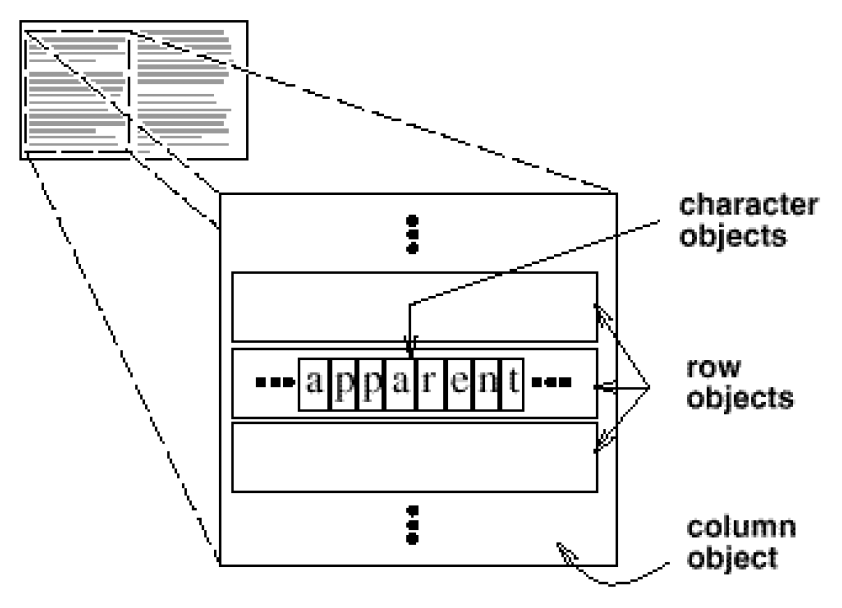
\includegraphics[scale=0.4]{motivation1.png}
\end{center}
\end{frame}
%-------------------------------------------------------------------------------------------------

%-------------------------------------------------------------------------------------------------
\begin{frame}\frametitle{Մոտիվացիան}
\begin{center}
    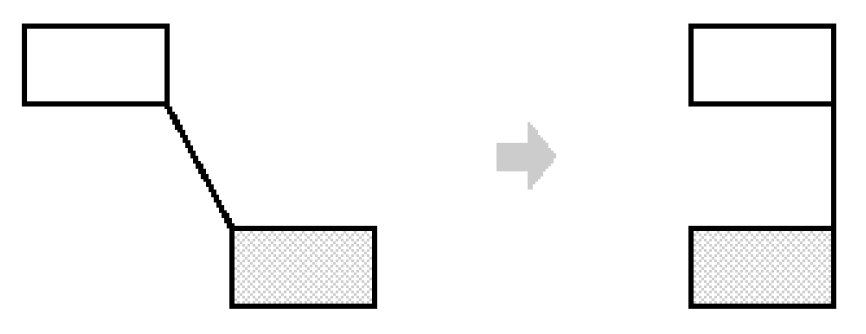
\includegraphics[scale=0.4]{motivation2.png}
\end{center}
\end{frame}
%-------------------------------------------------------------------------------------------------

\subsection{Կիրառելիությունը}
%-------------------------------------------------------------------------------------------------
\begin{frame}\frametitle{Կիրառելիությունը}
Այս Ն.Ձ. պետք է օգտագործել երբ.
\vfill
\begin{enumerate}
    \item Ցանկանում եք տրամադրել պարզ ինտերֆեյս կոմպլեքս ենթահամակարգի
    հետ աշխատելու համար: \pause \vfill
    \item Ցանկանում եք նվազեցնել ենթահամակարգի կախվածությունը օգտագործողից
    և այլ ենթահամակարգերից: \pause \vfill
    \item Ցանկանում եք շերտավորել ձեր ենթահամակարգերը:
\end{enumerate}
\end{frame}
%-------------------------------------------------------------------------------------------------

\section{Կառուցվածքը}
%-------------------------------------------------------------------------------------------------
\begin{frame}\frametitle{Կառուցվածքը}
\begin{center}
    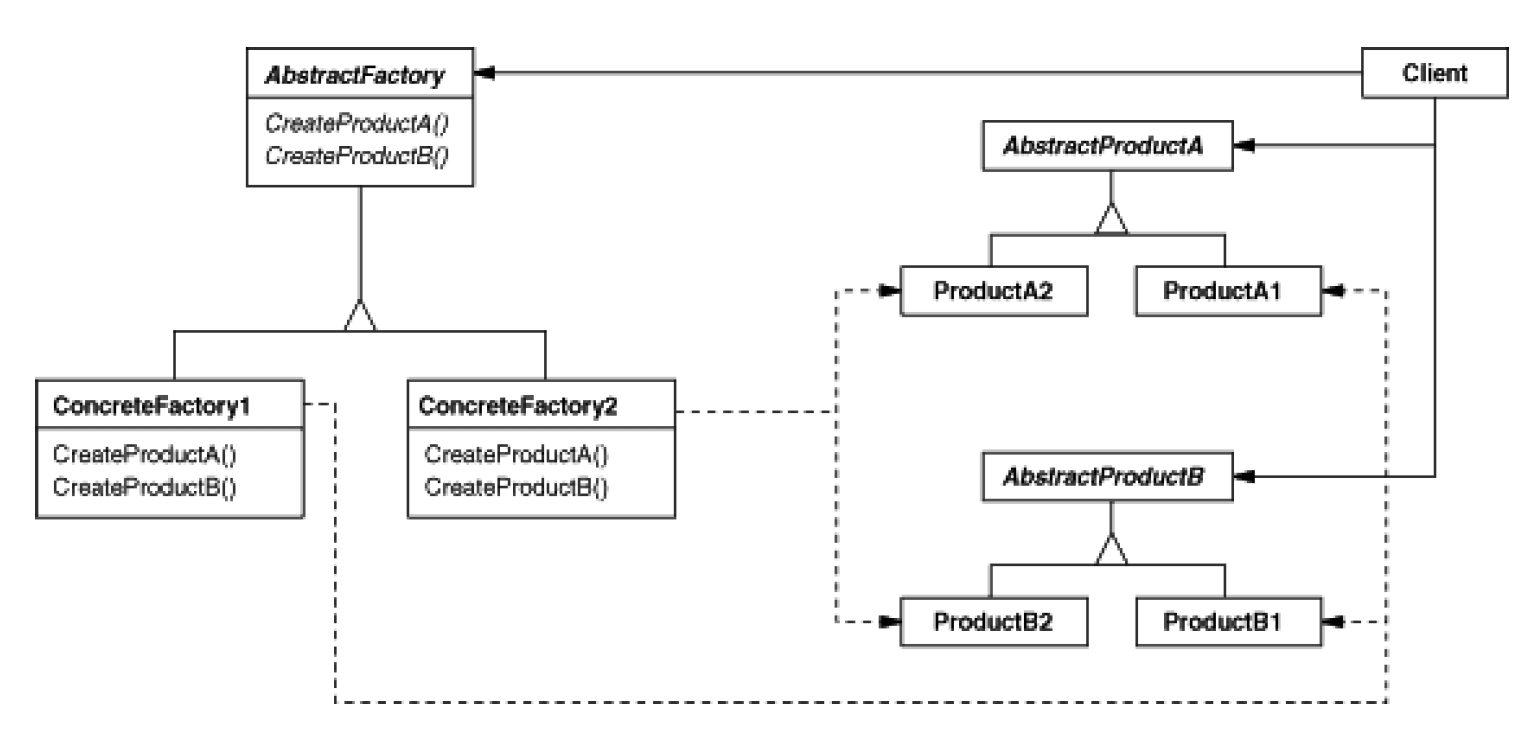
\includegraphics[scale=0.4]{structure.png}
\end{center}
\end{frame}
%-------------------------------------------------------------------------------------------------

\subsection{Հետևանքները}
%-------------------------------------------------------------------------------------------------
\begin{frame}\frametitle{Հետևանքները}
Այս Ն.Ձ. ունի հետևյալ առավելություններն ու թերությունները.
\vfill
\begin{enumerate}
    \item Նվազեցնում է այն օբյեկտների քանակը, որոնց հետ առնչվում է օգտագործողը,
    դարձնելով ենթահամակարգը հեշտ օգտագործելի: \pause \vfill
    \item Նվազեցնում է ենթահամակարգի կախվածությունը օգտագործողից և այլ
    ենթահամակարգերից: \pause \vfill
    \item Չի խոչդոտում օգտագործողի կողմից ենթահամակարգի դասերի օգտագործմանը
    (եթե դրա կարիքը կա): Այսինքն օգտագործողը կարող է որոշել ինչն է իրեն անհրաժեշտ
    ընդհանրությունը, թե պարզությունը:
\end{enumerate}
\end{frame}
%-------------------------------------------------------------------------------------------------

\section{Իրականացումը}
%-------------------------------------------------------------------------------------------------
\begin{frame}\frametitle{Իրականացումը}
\begin{enumerate}
    \item Հաճախորդներ-ենթահամակարգ կապերի կրճատում: \vfill
    \item public ենթահամակարգային դասերը ընդդեմ  private ենթահամակարգային դասերի:
\end{enumerate}
\end{frame}
%-------------------------------------------------------------------------------------------------

\subsection{Օրինակ}
%-------------------------------------------------------------------------------------------------
\begin{frame}[fragile]\frametitle{Օրինակ}
\begin{english}
\begin{minted}{cpp}
Scanner scanner(input);

ProgramNodeBuilder builder;

Parser parser;

parser.Parse(scanner, builder);

RISCCodeGenerator generator(output);

ProgramNode* parseTree = builder.GetRootNode();

parseTree->Traverse(generator);
\end{minted}
\end{english}
\end{frame}
%-------------------------------------------------------------------------------------------------
%-------------------------------------------------------------------------------------------------
\begin{frame}[fragile]\frametitle{Օրինակ}
\begin{english}
\begin{minted}{cpp}
class Compiler {

public:
    Compiler();

    virtual void Compile(istream& input, BytecodeStream& output) {

        Scanner scanner(input);
        ProgramNodeBuilder builder;
        Parser parser;
        parser.Parse(scanner, builder);
        RISCCodeGenerator generator(output);
        ProgramNode* parseTree = builder.GetRootNode();
        parseTree->Traverse(generator);
    }
};
\end{minted}
\end{english}
\end{frame}
%-------------------------------------------------------------------------------------------------

\section{Առնչվող Ձևանմուշները}
%-------------------------------------------------------------------------------------------------
\begin{frame}\frametitle{Առնչվող Նախագծման Ձևանմուշները}
\begin{itemize}
    \item Abstract Factory \vfill
    \item Mediator \vfill
    \item Singleton
\end{itemize}
\end{frame}
%-------------------------------------------------------------------------------------------------

\end{document}
